\documentclass[a4paper,12pt]{article}

% Package for Unicode support
\usepackage[utf8]{inputenc}
\usepackage{float}
\usepackage{placeins}
% Language and font encoding
\usepackage[utf8]{inputenc}
\usepackage[english]{babel} % English language support
\usepackage{amsmath}
% Geometry package for page margins
\usepackage{geometry}
\geometry{
 a4paper,
 total={170mm,257mm},
 left=25mm,
 right=25mm,
 top=25mm,
 bottom=25mm
}

% For math symbols and equations
\usepackage{amsmath}
\usepackage{siunitx}
\usepackage{caption}
\usepackage{booktabs}

% Graphicx for including images
\usepackage{graphicx}
\graphicspath{{figures/}}

% Hyperlink support with hidden links
\usepackage[hidelinks]{hyperref}


% Package for professional tables
\usepackage{booktabs}

% Package for fancy header and footer
\usepackage{fancyhdr}
\pagestyle{fancy}
\fancyhf{}
\fancyhead[L]{ATCS} % Module name in header
\fancyhead[R]{\leftmark} % Section title in header
\fancyfoot[C]{\thepage} % Page number in the footer

% For including code snippets
\usepackage{listings}
\lstset{
    basicstyle=\ttfamily,
    breaklines=true
}

% Title page formatting
\title{
    \vspace{2cm}
    \textbf{Drone Control}\\
    \large Course: Advanced Techniques of Control Systems\\
    \vspace{1cm}
}
\author{
    Stylianos Bouliaris-Malatestas\\
    Student ID: 03119214\\
    \vspace{0.5cm}
    National Technical University of Athens (NTUA)\\
    School of Electrical and Computer Engineering
}
\date{\today}

% Begin Document
\begin{document}

% Title page
\maketitle
\thispagestyle{empty}
\newpage

% Table of contents
\tableofcontents
\newpage

% Section 1: Introduction
\section{Introduction}
In this assignment we deal with the control of a drone (quadrotor). Specifically, we will test different control methods, such as PID, Cascaded PID, and state-space control using LQR. In the end, we will attempt to assign a trajectory to the drone using the controllers we have designed, and we will observe how our system responds. Our drone is shown in the figure below:
% Insert an image
\begin{figure}[h] % 'h' places the image approximately where it appears in the code
    \centering
    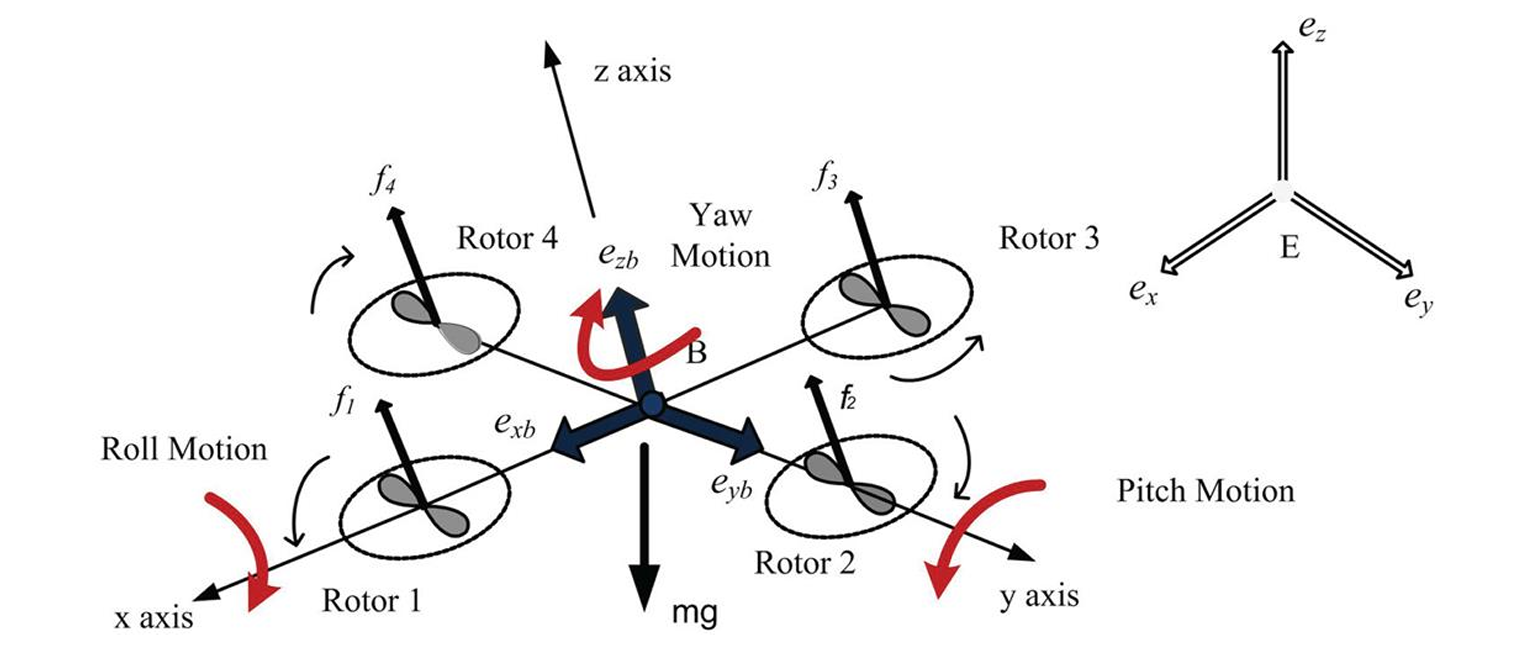
\includegraphics[width=0.9\textwidth]{DroneSchematic.png} % Specify image file and width
    \caption{Quadrotor Drone System} % Image caption
    \label{fig:DroneSchematic} % Label for referencing the image
\end{figure}
\newline
Our drone has 6 degrees of freedom: 3 rotations, roll, pitch, yaw ($\phi, \theta, \psi$), and 3 translations ($x, y, z$). Obviously, the rotational speed of the motors (and hence the lift force produced by each motor) affects the state variables of the drone that we have just described.

\newpage







% Section 2: Theory
\section{System Modeling}
\subsection{Description of Rotational Motion}
The drone has 4 rotors. Two of them rotate clockwise (the rotors along the axis through which the x' axis passes) and the other two rotate counter-clockwise. Thus, in hovering mode, where it stays fixed at a point, the total angular momentum of the rotors is 0. The thrust produced by each rotor ($i=1,2,3,4$) is proportional to the square of its angular velocity and is given by the relation:
\begin{equation}
    f_i = b\Omega_i^2
\end{equation}
To make the drone rotate about the x-axis (roll motion, change of the angle $\phi$), the speed of rotor 2 is initially decreased and that of rotor 4 is increased, which creates a torque about the x-axis, which in turn produces an angular velocity (obviously, to stop this angular motion an opposite torque is required). Similarly, the rotation about the y-axis is achieved through the difference in the speeds of rotors 1 and 3. The rotation about the z-axis is achieved by increasing the speed of two diametrically opposite rotors and decreasing that of the other pair (the torque is achieved through the drag resistance to the rotors' motion).
\subsection{Description of Translational Motion}
In order for the drone to move along the z-axis, the total force along that axis must be greater than its weight. The force is described by the relation:
\begin{equation}
    U_1 = b(\Omega_1^2+\Omega_2^2+\Omega_3^2+\Omega_4^2)
\end{equation}
For motion to occur along the x and y axes, the drone must first rotate about the y (pitch) and x (roll) axes respectively, so that a component of the total force $U_1$ appears along the axis on which we want motion to occur. Therefore, the following relations express:
\begin{equation}
    U_2 = b(\Omega_4^2 - \Omega_2^2),  \quad \textrm{$U_2$ controls the motion along the x-axis}
\end{equation}

\begin{equation}
    U_3 = b(\Omega_3^2 - \Omega_1^2),  \quad \textrm{$U_3$ controls the motion along the y-axis}
\end{equation}

\begin{equation}
    U_4 = d(\Omega_1^2+\Omega_3^2-\Omega_2^2-\Omega_4^2),  \quad \textrm{$U_4$ controls the rotation about z}
\end{equation}
\newline
Note that $U_1,U_2,U_3$ depend on the thrust factor $b$, while $U_4$ depends on the drag factor $d$.
\newpage
\subsection{Mathematical Modeling in State Space}
The state variables we need in order to describe the system are none other than the Euler angles $\phi, \theta, \psi$ about the axes, as well as the translations $x, y, z$ along those axes. The state equations for the rotational motions are the following:
\begin{equation}
    \Ddot{\phi} = \dot{\theta}\dot{\psi}[\frac{I_{yy}-I_{zz}}{I_{xx}}] + \frac{1}{I_{xx}}U_2
\end{equation}

\begin{equation}
    \Ddot{\theta} = \dot{\phi}\dot{\psi}[\frac{I_{yy}-I_{xx}}{I_{yy}}] + \frac{1}{I_{yy}}U_3
\end{equation}

\begin{equation}
    \Ddot{\psi} = \dot{\theta}\dot{\phi}[\frac{I_{xx}-I_{yy}}{I_{zz}}] + \frac{1}{I_{zz}}U_4
\end{equation}
\newline
The motion along the $x, y, z$ axes is given by the equations:
\begin{equation}
    \Ddot{x} = (c_{\phi}s_{\theta}c_{\psi} + s_{\phi}s_{\psi})\frac{1}{m}U_1
\end{equation}

\begin{equation}
    \Ddot{y} = (-c_{\phi}s_{\theta}s_{\psi} + s_{\phi}c_{\psi})\frac{1}{m}U_1
\end{equation}

\begin{equation}
    \Ddot{z} = -g +(c_{\phi}c_{\theta})\frac{1}{m}U_1
\end{equation}
\newline
\noindent
In the above equations, the terms $c_{i}, s_{i}$ are abbreviations for $cos(i), sin(i)$. For the remainder of the assignment, we take the values of the variables appearing in the above equations according to Table $(1)$. We will further assume that each rotor can rotate at a maximum speed of $\Omega_{max} = 15000 RPM$

\begin{table}[h!]
\centering
\caption{Physical parameters of the quadrotor system.}
\begin{tabular}{lll}
\toprule
\textbf{Parameter} & \textbf{Symbol} & \textbf{Value} \\
\midrule
Total weight of the vehicle         & \( m \)   & 0.800 kg \\
Gravitational acceleration          & \( g \)   & 9.81
\(\si{\meter\per\second\squared}\) \\
Arm length of the vehicle           & \( l \)   & 0.3 m \\
Moment of inertia along x-axis      & \( I_{xx} \) & \( 15.67 \times 10^{-3} \, \si{\kilogram\meter\squared} \) \\
Moment of inertia along y-axis      & \( I_{yy} \) & \( 15.67 \times 10^{-3} \, \si{\kilogram\meter\squared} \) \\
Moment of inertia along z-axis      & \( I_{zz} \) & \( 28.34 \times 10^{-3} \, \si{\kilogram\meter\squared} \) \\
Thrust factor                       & \( b \)   & \( 192.32 \times 10^{-7} \, \si{\newton\second\squared} \) \\
Drag factor                         & \( d \)   & \( 4.003 \times 10^{-7} \, \si{\newton\meter\second\squared} \) \\
\bottomrule
\end{tabular}
\end{table}
\newpage









% Section 3 Control
\section{Cascaded PID Control}
\subsection{Elimination of the angles $\phi, \theta$ and keeping the drone at a constant altitude}\label{3.1}
Our goal is to stabilize the angles $\phi, \theta$ at $0$ while keeping the drone's altitude at a specific desired value. We chose the following initial conditions:
\begin{table}[h!]
\centering
\caption{Initial Conditions}
\begin{tabular}{|c|c|c|}
\hline
\textbf{Variable Name} & \textbf{Symbol} & \textbf{Value} \\ \hline
Initial $\phi$ & $\phi_0$ & $0.02 rad$ \\ \hline
Initial $\theta$ & $\theta_0$  & $0.02 rad$ \\ \hline
Initial $z$ & $z_0$  & $0 m$ \\ \hline
\end{tabular}
\end{table}

\noindent
We therefore build a PID controller for each of the inputs $U_1, U_2, U_3$, since these are responsible for the motions we want to control. After several trials, we conclude that the ideal gains for the controllers are:
\begin{equation}
    [K_p = 1, K_i = 0.5, K_d = 4],   \quad \textrm{For $U_1$}
\end{equation}
\begin{equation}
    [K_p = 2, K_i = 0, K_d = 0.35],   \quad \textrm{For $U_2, U_3$}
\end{equation}
\noindent
Below we see the response of the drone using the above controllers, when we set the desired value for $z = 1m$
\begin{figure}[h!] % 'h' places the image approximately where it appears in the code
    \centering
    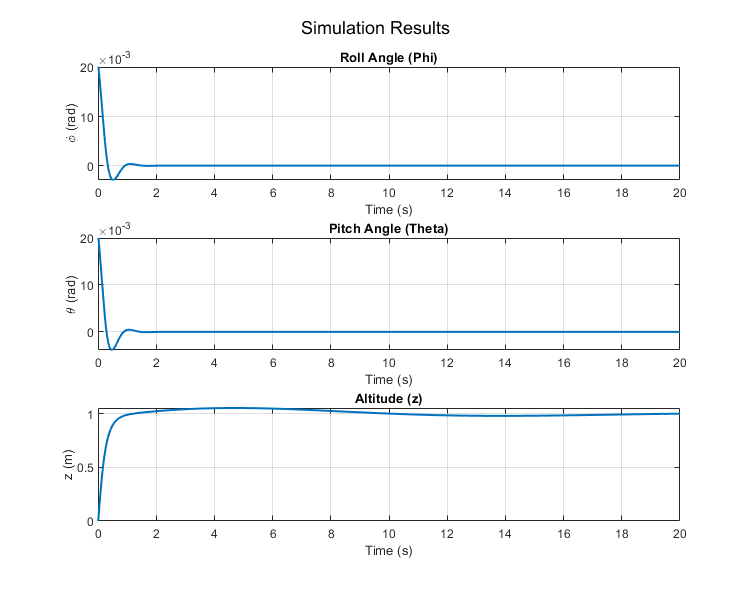
\includegraphics[width=0.8\textwidth]{DroneResponsePID.png} % Specify image file and width
    \caption{Response with gains specified in $(12), (13), (14)$ for $z_{d} = 1$} % Image caption
    \label{fig:DroneResponsePID} % Label for referencing the image
\end{figure}
\newline
We see that our system responds quite quickly and settles into the steady state as desired.
\subsection{Control of $x, y, z$ to desired values, using Cascaded PID}\label{3.2}
The goal now is for our drone to reach a desired point, with coordinates $x, y, z$ in Cartesian space. To do this, we will design 2 Cascaded PID controllers for the $x$ and $y$ position and we will use the controller we designed previously to stabilize the drone at a specific $z$. The coordinates of the point we want to reach are:
 \begin{table}[h!]
\centering
\caption{Desired Coordinates}
\begin{tabular}{|c|c|c|}
\hline
\textbf{Variable Name} & \textbf{Symbol} & \textbf{Value} \\ \hline
Desired $x$ & $x_d$  & $1m$ \\ \hline
Desired $y$ & $y_d$  & $4m$ \\ \hline
Desired $z$ & $z_d$  & $4m$ \\ \hline
\end{tabular}
\end{table}
\begin{figure}[h!] % 'h' places the image approximately where it appears in the code
    \centering
    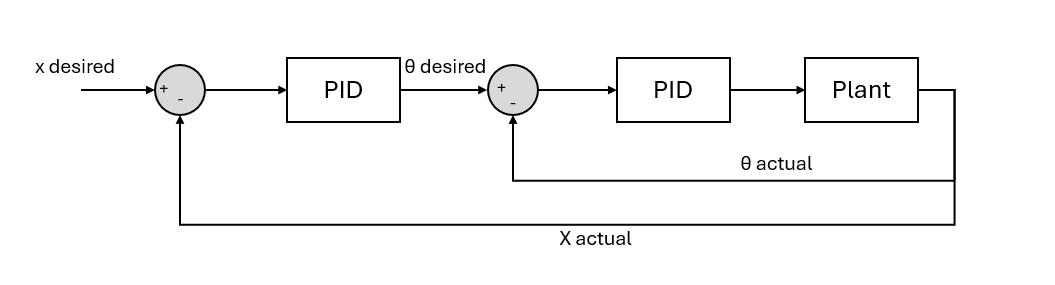
\includegraphics[width=1\textwidth]{CascadedControllerBlockDiagram.png} % Specify image file and width
    \caption{Block diagram of Cascaded PID for $\theta$} % Image caption
    \label{fig:CascadedBlockDiagram} % Label for referencing the image
\end{figure}

\noindent
It was deemed appropriate to first wait for the drone to stabilize at the desired altitude, and then command it to move to the desired $x$ and $y$. After several trials, the gains used in the Cascaded PID controllers are:
\begin{equation}
    [K_p = 1, K_i = 0, K_d = 0.7],   \quad \textrm{For computing the desired angle}
\end{equation}

\begin{equation}
    [K_p = 2.95, K_i = 0.5, K_d = 2.6],   \quad \textrm{For controlling the motors}
\end{equation}

\noindent
In addition, it is important to note that directly controlling the angles $\phi, \theta$ using the global coordinates $x$ and $y$ does not work, because we are not yet controlling the angle $\psi$; therefore, when the drone rotates, its axes cease to coincide with the inertial global reference frame.
\newline
\newline
The transformation into the drone's reference frame is performed as follows:
\begin{equation}
    x_{drone} = xcos(\psi)+ysin(\psi)
\end{equation}

\begin{equation}
    y_{drone} = ycos(\psi)-xsin(\psi)
\end{equation}
\newpage
\noindent
Below we see the response of the drone using the control system we described. It is important to note that we have limited the outputs of the PIDs that compute the desired angles (according to the position deviation) to the interval $\phi,\theta \in [-15, 15]$, aiming to avoid large target angles that could possibly drive the system into instability.
\begin{figure}[h!] % 'h' places the image approximately where it appears in the code
    \centering
    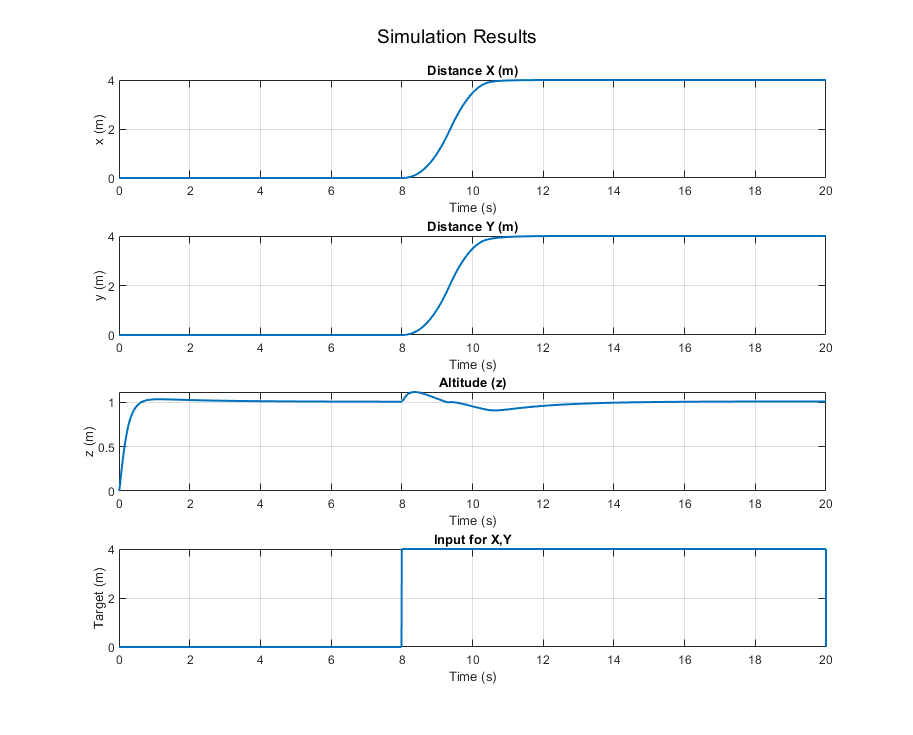
\includegraphics[width=1\textwidth]{DroneResponseCPID_disp.png} % Specify image file and width
    \caption{Drone position \& Controller input } % Image caption
    \label{fig:DroneResponseCPID_disp} % Label for referencing the image
\end{figure}
\newline
We observe that when the drone begins to move along the $x$ and $y$ axes, the altitude overshoots, which is not easy to compensate for quickly, since we cannot exert a downward force but can only reduce the lift, letting gravity correct the overshoot. However, we observed that this particular overshoot during the initial acceleration, as well as the undershoot during the deceleration, are directly connected to the angle limits we allow the drone. Thus, the angle limits we discussed above constitute a compromise between response speed and error in the $z$ position.
\newline
\newline
Next we see the angular response of the drone. Initially the goal is to stabilize at altitude $z = 1$, which does not affect the angles. At 8 seconds, once the drone has stabilized, it begins to follow the targets for the $x$ and $y$ coordinates. We therefore expect to observe a change in the angles $\phi, \theta$.
\begin{figure}[h!] % 'h' places the image approximately where it appears in the code
    \centering
    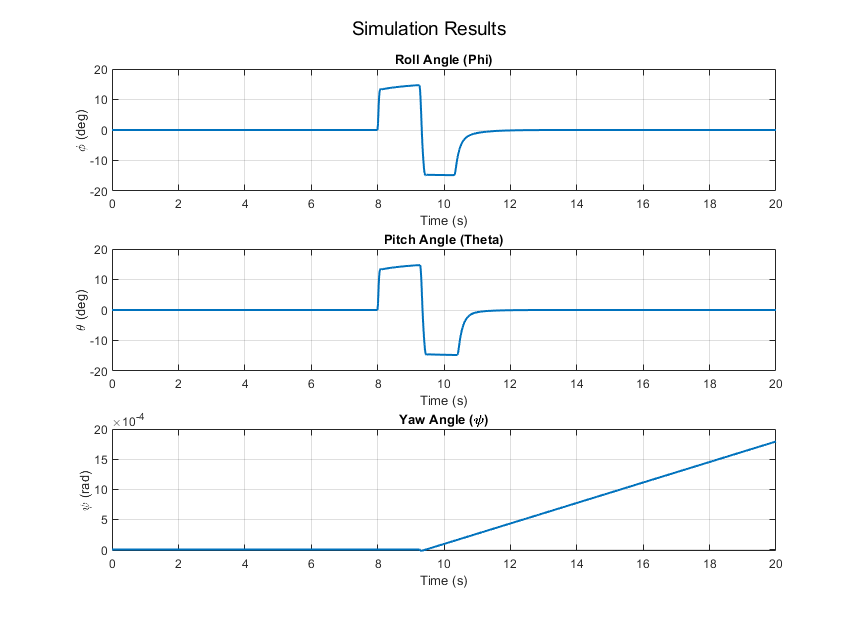
\includegraphics[width=1\textwidth]{DroneResponseCPID.png} % Specify image file and width
    \caption{Drone Euler angles } % Image caption
    \label{fig:DroneResponseCPID} % Label for referencing the image
\end{figure}
\newpage
\noindent
We observe that the yaw angle ($\psi$) does not change and remains practically constant, despite the fact that we do not control it. This is due to the fact that the targets and controllers for the angles $\phi, \theta$ are identical, so by issuing the same speed command the yaw torques cancel out. The speed diagrams of each rotor are shown in figure \ref{fig:Drone_Angular_Velocities}.
\newline
\newline
It is also worth noting that although the same controller was used as in \ref{3.1}, its gains needed adjustment, in order to reduce the maximum error in the transient state. The new gains are shown below:
\begin{equation}
    [K_p = 2, K_i = 0.1, K_d = 4.4],   \quad \textrm{For $U_1$}
\end{equation}
\begin{figure}[h!] % 'h' places the image approximately where it appears in the code
    \centering
    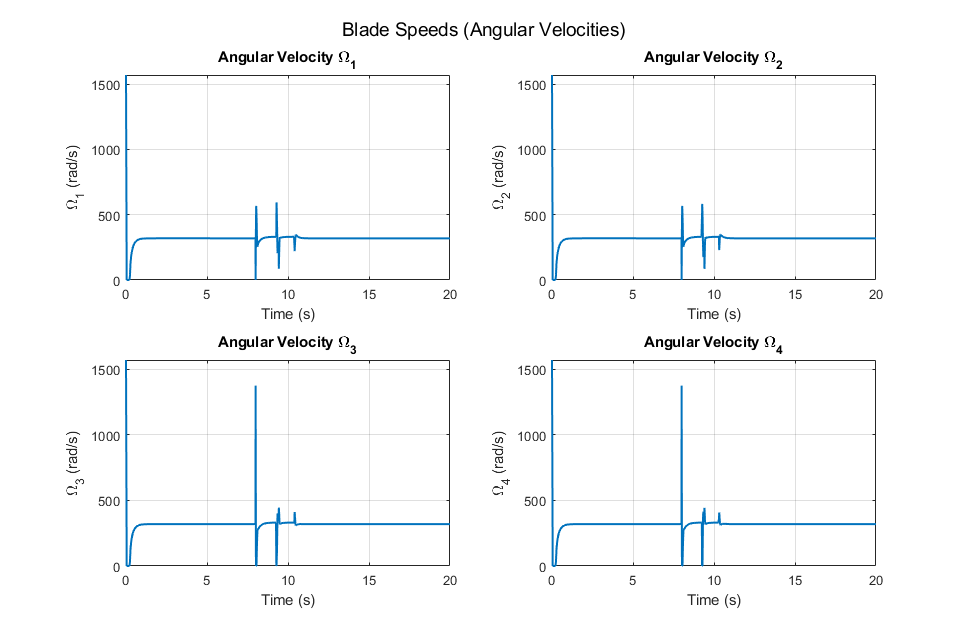
\includegraphics[width=1\textwidth]{Drone_Angular_Velocities.png} % Specify image file and width
    \caption{Drone angular velocities } % Image caption
    \label{fig:Drone_Angular_Velocities_plot} % Label for referencing the image
\end{figure}
\newpage
\subsection{Control of $x, y, z$ as well as $\psi$ to desired values, using Cascaded PID}
The goal now is to perform the control of question \ref{3.2} while at the same time also controlling the yaw angle ($\psi$). To achieve this we will keep the controller concept described previously, and we will additionally implement a simple PID that will control the yaw. If needed, changes will also be made to the other controllers to improve the combined performance of the system.
\newline
\newline
After several trials we arrive at the following gains for the controllers. We observe that only very small changes were needed, and not for all controllers. Furthermore, for controlling the yaw angle we used the same controller that is responsible for controlling the motors in the Cascaded PID.
\begin{equation}
    [K_p = 2, K_i = 0.1, K_d = 4.4],   \quad \textrm{For $U_1$}
\end{equation}

\begin{equation}
    [K_p = 1, K_i = 0, K_d = 1.05],   \quad \textrm{For computing the desired angle}
\end{equation}

\begin{equation}
    [K_p = 2.95, K_i = 0.5, K_d = 2.6],   \quad \textrm{For controlling the motors}
\end{equation}

\begin{equation}
    [K_p = 2.95, K_i = 0.5, K_d = 2.6],   \quad \textrm{For $U_4$}
\end{equation}

\newpage
\noindent
The system response is shown below. It is worth noting that this time the targets for the $x$ and $y$ position are set with a time difference of 1 second, in order to make the role of the yaw controller even more difficult.
\begin{figure}[h!] % 'h' places the image approximately where it appears in the code
    \centering
    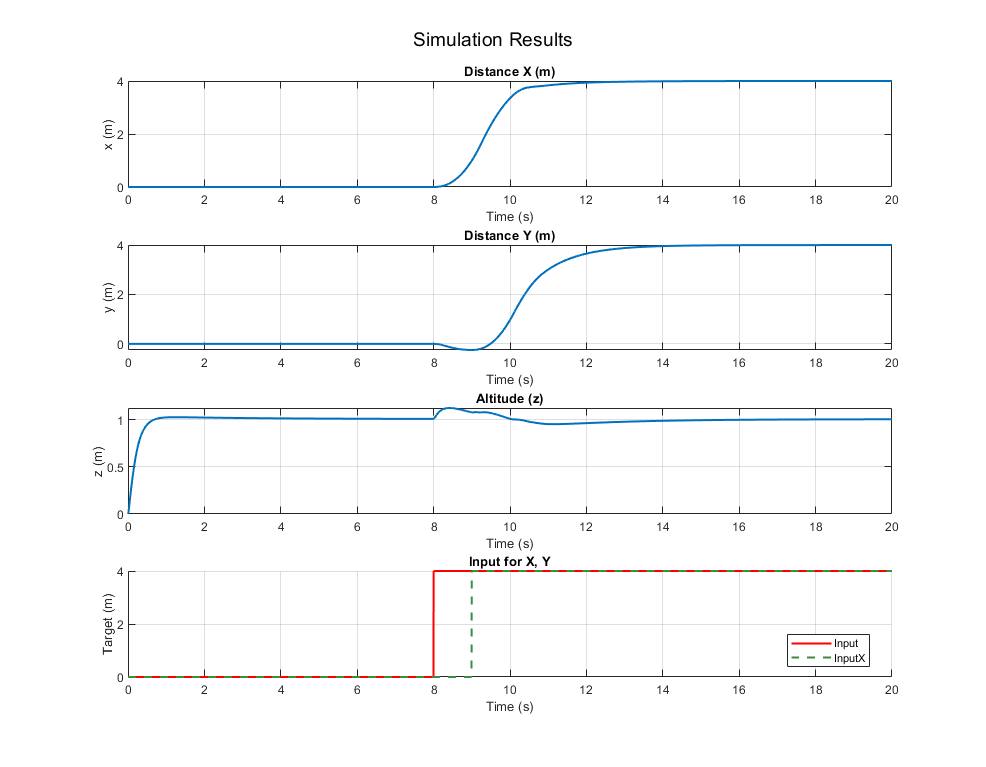
\includegraphics[width=1\textwidth]{DroneResponseCPID_disp_to_follow_psi.png} % Specify image file and width
    \caption{Drone position \& Controller input  } % Image caption
    \label{fig:Drone_Angular_Velocities} % Label for referencing the image
\end{figure}
\newline
We observe that despite the increased complexity of the control problem, our controllers manage to drive the drone effectively to the equilibrium points we set as targets. The effect of the yaw angle controller is perceptible in figure \ref{fig:Drone_Angular_Velocities_follow_psi}. Specifically, we see the rotor speeds increase and decrease in such a way that the altitude is not affected at all, giving the drone the appropriate speed to follow the desired angle. When the angle target finally stops changing, we observe the opposite behavior from the system so that it ceases to rotate.
\newline
\newline
Figure \ref{fig:Drone_Euler_Angles_follow_psi} shows that our controller responds very quickly and with minimal overshoot.
\FloatBarrier
\begin{figure}[H] % 'h' places the image approximately where it appears in the code
    \centering
    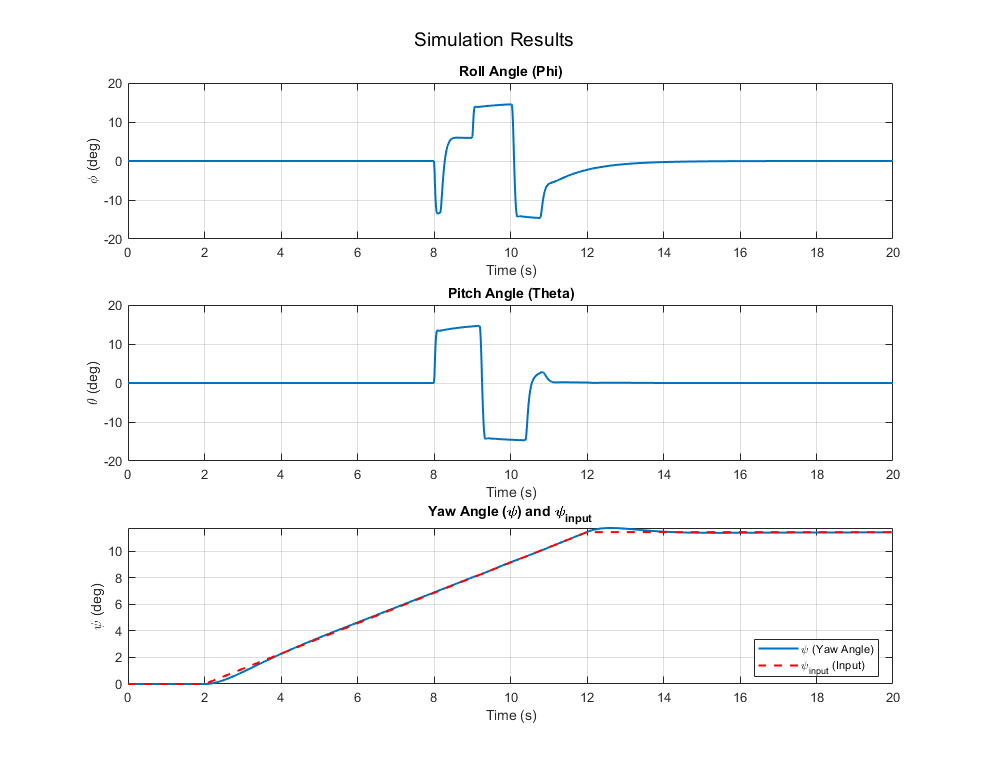
\includegraphics[width=0.84\textwidth]{DroneResponseCPID_to_follow_psi.png} % Specify image file and width
    \caption{Drone Euler angles } % Image caption
    \label{fig:Drone_Euler_Angles_follow_psi} % Label for referencing the image
\end{figure}
\vspace{1em}
\begin{figure}[h!] % 'h' places the image approximately where it appears in the code
    \centering
    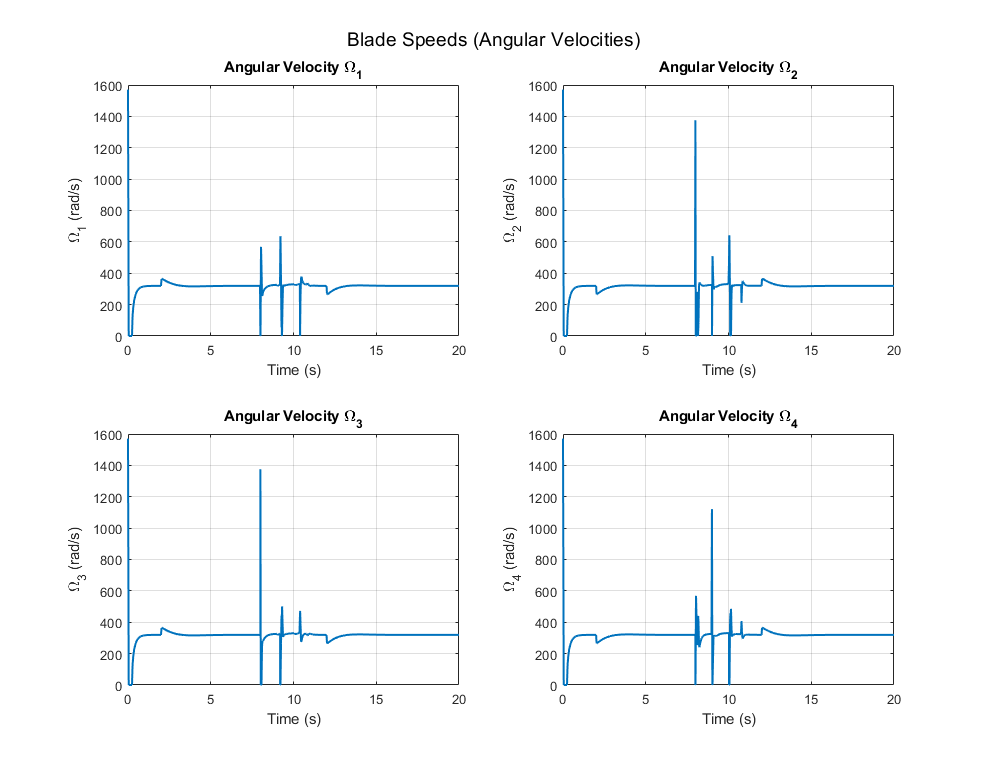
\includegraphics[width=0.84\textwidth]{Drone_Angular_Velocities_to_follow_psi.png} % Specify image file and width
    \caption{Drone angular velocities } % Image caption
    \label{fig:Drone_Angular_Velocities_follow_psi} % Label for referencing the image
\end{figure}
\clearpage
\section{State-Space Control}
\subsection{Computation of the equilibrium points}
To compute the equilibrium points it suffices to require that the relation hold, in which we define $s$ as the state vector $[x, y, z, \phi, \theta, \psi]$. It is also clear that for the system to be in equilibrium the angles $\theta$ and $\phi$ must be 0. If this were not the case, and the drone had an altitude $z > 0$, then it would not be in equilibrium.
\begin{equation}
    \frac{ds}{dt} = 0
\end{equation}
\newline
The state equations, therefore, assuming $\theta = 0$ and $\phi = 0$, are written as follows:
\begin{equation}
    \Ddot{x} = 0
\end{equation}

\begin{equation}
    \Ddot{y} = 0
\end{equation}

\begin{equation}
    \Ddot{z} = 0 \longrightarrow U_1 = mg
\end{equation}


\begin{equation}
    \Ddot{\phi} = 0
\end{equation}

\begin{equation}
    \Ddot{\theta} = 0
\end{equation}

\begin{equation}
    \Ddot{\psi} = 0
\end{equation}
We therefore conclude that any point in Cartesian space can constitute an equilibrium point, provided that the total thrust force is equal to the weight of the drone.
\subsection{Linearization around an equilibrium point}
First, in order to linearize this particular system, we must express it as a system of first-order differential equations. The dynamics of the system are therefore written as follows:
\begin{align*}
\dot{x}_1 &= x_2, \\
\dot{x}_2 &= p_1 x_4 x_6 + p_2 U_2, \\
\dot{x}_3 &= x_4, \\
\dot{x}_4 &= p_3 x_2 x_6 + p_4 U_3, \\
\dot{x}_5 &= x_6, \\
\dot{x}_6 &= p_5 x_2 x_4 + p_6 U_4, \\
\dot{x}_7 &= x_8, \\
\dot{x}_8 &= \left( c_\phi s_\theta c_\psi + s_\phi s_\psi \right) \frac{1}{m} U_1, \\
\end{align*}
\begin{align*}
\dot{x}_9 &= x_{10}, \\
\dot{x}_{10} &= \left( -c_\phi s_\theta s_\psi + s_\phi c_\psi \right) \frac{1}{m} U_1, \\
\dot{x}_{11} &= x_{12}, \\
\dot{x}_{12} &= -g + \left( c_\theta c_\phi \right) \frac{1}{m} U_1,
\end{align*}
We choose to linearize around the equilibrium point with Cartesian coordinates $(x,y,z) = (1, 1, 1)$ and Euler angles $(\phi, \theta, \psi) = (0, 0, 0)$. Now that our system has the appropriate form and we know the points of interest, we can compute the matrices A and B of the first-order linear system from the relation:
\begin{equation}
    \dot{x} = \frac{\partial f(x,u)}{\partial x} (x - x_{ss}) + \frac{\partial f(x,u)}{\partial u} (u - u_{ss})
\end{equation}
\begin{equation}
    A = \frac{\partial f(x,u)}{\partial x},  \quad  B = \frac{\partial f(x,u)}{\partial u}
\end{equation}
It follows that the matrices A and B are equal to:
\setcounter{MaxMatrixCols}{12}
\begin{equation}
A =
\begin{bmatrix}
 0 & 1 & 0 & 0 & 0 & 0 & 0 & 0 & 0 & 0 & 0 & 0 \\
0 & 0 & 0 & 0 & 0 & 0 & 0 & 0 & 0 & 0 & 0 & 0 \\
0 & 0 & 0 & 1 & 0 & 0 & 0 & 0 & 0 & 0 & 0 & 0 \\
0 & 0 & 0 & 0 & 0 & 0 & 0 & 0 & 0 & 0 & 0 & 0 \\
0 & 0 & 0 & 0 & 0 & 1 & 0 & 0 & 0 & 0 & 0 & 0 \\
0 & 0 & 0 & 0 & 0 & 0 & 0 & 0 & 0 & 0 & 0 & 0 \\
0 & 0 & 0 & 0 & 0 & 0 & 0 & 1 & 0 & 0 & 0 & 0 \\
0 & 0 & 9.81 & 0 & 0 & 0 & 0 & 0 & 0 & 0 & 0 & 0 \\
9.81 & 0 & 0 & 0 & 0 & 0 & 0 & 0 & 0 & 0 & 0 & 0 \\
0 & 0 & 0 & 0 & 0 & 0 & 0 & 0 & 0 & 1 & 0 & 0 \\
0 & 0 & 0 & 0 & 0 & 0 & 0 & 0 & 0 & 0 & 0 & 1 \\
0 & 0 & 0 & 0 & 0 & 0 & 0 & 0 & 0 & 0 & 0 & 0 \\
\end{bmatrix}
\end{equation}


\begin{equation*}
B =
\begin{bmatrix}
0 & 0 & 0 & 0 \\
0 & 19.1449 & 0 & 0 \\
0 & 0 & 0 & 0 \\
0 & 0 & 19.1449 & 0 \\
0 & 0 & 0 & 0 \\
0 & 0 & 0 & 35.2858 \\
0 & 0 & 0 & 0 \\
0 & 0 & 0 & 0 \\
0 & 0 & 0 & 0 \\
0 & 0 & 0 & 0 \\
0 & 0 & 0 & 0 \\
1.25 & 0 & 0 & 0 \\
\end{bmatrix}
\end{equation*}

\newpage
\subsection{Computation of the transfer matrix from input to output (with outputs $x, y, z, \psi$)}
Our system is a MIMO system (Multiple Input Multiple Output). Consequently, a single transfer function is not defined, but rather a matrix of transfer functions from the inputs to the outputs. By computing this matrix for the linearized system, we can understand how each input affects the output, as well as which inputs affect which outputs, making the tuning process easier during controller design.

\noindent
Using the appropriate MATLAB functions to avoid errors in the calculations, we computed the transfer matrix:
\begin{equation*}
G =
\begin{bmatrix}
\frac{1.25}{s^2} & 0 & 0 & 0\\
0 & \frac{187.8}{s^4} & 0 & 0\\
0 & 0 & \frac{187.8}{s^4} & 0\\
0 & 0 & 0 & \frac{35.2858}{s^2}\\
\end{bmatrix}
\end{equation*}
\noindent
For the above transfer matrix the following holds:
\begin{equation*}
\begin{bmatrix}
    z\\
    y\\
    x\\
    \psi\\
\end{bmatrix} =
\begin{bmatrix}
\frac{1.25}{s^2} & 0 & 0 & 0\\
0 & \frac{187.8}{s^4} & 0 & 0\\
0 & 0 & \frac{187.8}{s^4} & 0\\
0 & 0 & 0 & \frac{35.2858}{s^2}\\
\end{bmatrix}
\begin{bmatrix}
    U_1\\
    U_2\\
    U_3\\
    U_4\\
\end{bmatrix}
\end{equation*}
We observe that the transfer matrix is diagonal. This happens because we chose to linearize the system around a yaw angle $\psi = 0$, which allows the decoupling of $x$ and $y$. We also see that the position along the $x$-axis is affected by the pitch angle, and correspondingly the position along $y$ by the roll angle; that is, the position along $x$ depends on the rotation about $y$ and correspondingly the position $y$ on the rotation about $x$. This is a useful observation to express mathematically as well, because in systems for which we do not have such an easy empirical understanding, such things may not be so self-evident. We also observe that, since the inputs $U_2, U_3$ do not affect the outputs directly, but affect them through the angles as we discussed previously, 4 integrators are needed ($s^4$ in the denominator). By contrast, $U_1, U_4$ affect their variables directly, so only 2 integrators are needed.
\newline
\newline
Obviously these observations hold for the linearized system, so it becomes clear that the real system will not exhibit exactly these characteristics.
\newpage
\subsection{Controller design with LQR and testing on a specific trajectory}
Now that we have linearized the system and gained some understanding of how the outputs relate to the inputs, we can use classical tools for designing linear controllers for linear systems in state space. Specifically, we will use an LQR in order to compute the controller gains.
\newline
\newline
But let us first describe the control law with a block diagram. Previously we used 4 cascaded PID controllers, one for each input. Now, by solving the Riccati equation for chosen Q and R matrices, we will arrive at a gain matrix and apply the control law described by the block diagram below.
\begin{figure}[H] % 'h' places the image approximately where it appears in the code
    \centering
    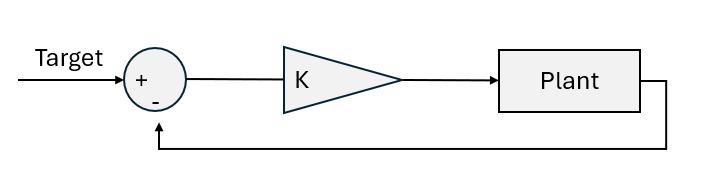
\includegraphics[width=0.84\textwidth]{LQR_Control.png} % Specify image file and width
    \caption{LQR Control law} % Image caption
    \label{fig:LQR_control} % Label for referencing the image
\end{figure}
\noindent
As with the tuning of the PID controllers, in order to find the most suitable Q, R matrices we followed a trial-and-error procedure. After many trials, where again our goal was fast system response as well as minimization of the deviation from the desired state, we arrived at the following matrices:
\begin{equation}
Q =
\begin{bmatrix}
3 & 0 & 0 & 0 & 0 & 0 & 0 & 0 & 0 & 0 & 0 & 0 \\
0 & 0.01 & 0 & 0 & 0 & 0 & 0 & 0 & 0 & 0 & 0 & 0 \\
0 & 0 & 3 & 0 & 0 & 0 & 0 & 0 & 0 & 0 & 0 & 0 \\
0 & 0 & 0 & 0.01 & 0 & 0 & 0 & 0 & 0 & 0 & 0 & 0 \\
0 & 0 & 0 & 0 & 3 & 0 & 0 & 0 & 0 & 0 & 0 & 0 \\
0 & 0 & 0 & 0 & 0 & 0.1 & 0 & 0 & 0 & 0 & 0 & 0 \\
0 & 0 & 0 & 0 & 0 & 0 & 1 & 0 & 0 & 0 & 0 & 0 \\
0 & 0 & 0 & 0 & 0 & 0 & 0 & 0.2 & 0 & 0 & 0 & 0 \\
0 & 0 & 0 & 0 & 0 & 0 & 0 & 0 & 1 & 0 & 0 & 0 \\
0 & 0 & 0 & 0 & 0 & 0 & 0 & 0 & 0 & 0.2 & 0 & 0 \\
0 & 0 & 0 & 0 & 0 & 0 & 0 & 0 & 0 & 0 & 15 & 0 \\
0 & 0 & 0 & 0 & 0 & 0 & 0 & 0 & 0 & 0 & 0 & 1 \\
\end{bmatrix}
\end{equation}


\begin{equation*}
R =
\begin{bmatrix}
1 & 0 & 0 & 0\\
0 & 0.1 & 0 & 0\\
0 & 0 & 0.1 & 0\\
0 & 0 & 0 & 0.1\\
\end{bmatrix}
\end{equation*}
\newpage
\begin{figure}[H] % 'h' places the image approximately where it appears in the code
    \centering
    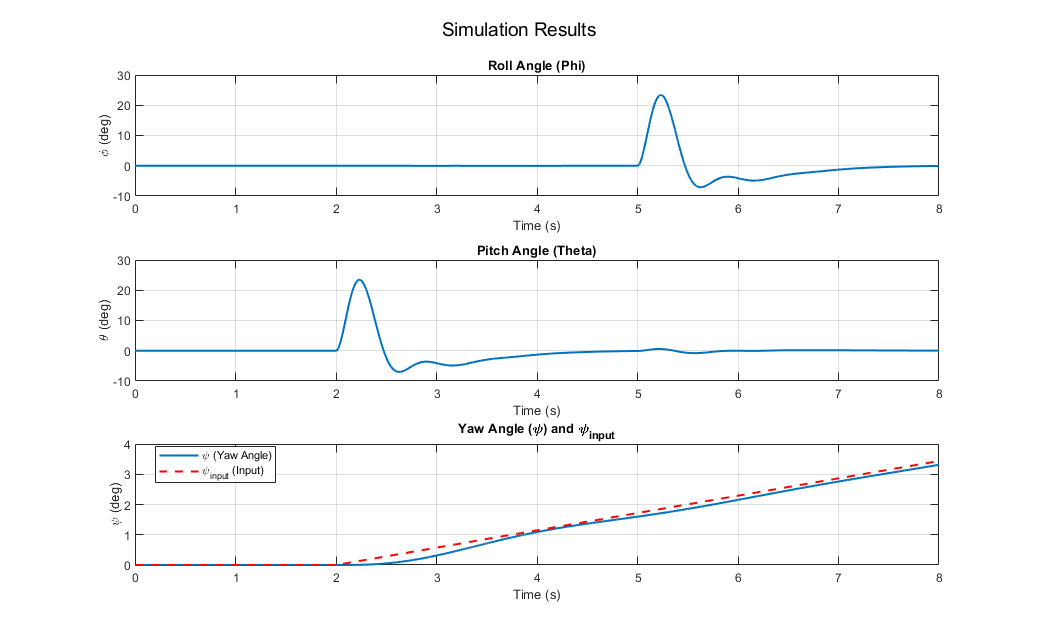
\includegraphics[width=1\textwidth]{LQR_Angles.png} % Specify image file and width
    \caption{LQR controller Euler angle response} % Image caption
    \label{fig:LQR_Angles} % Label for referencing the image
\end{figure}
\begin{figure}[H] % 'h' places the image approximately where it appears in the code
    \centering
    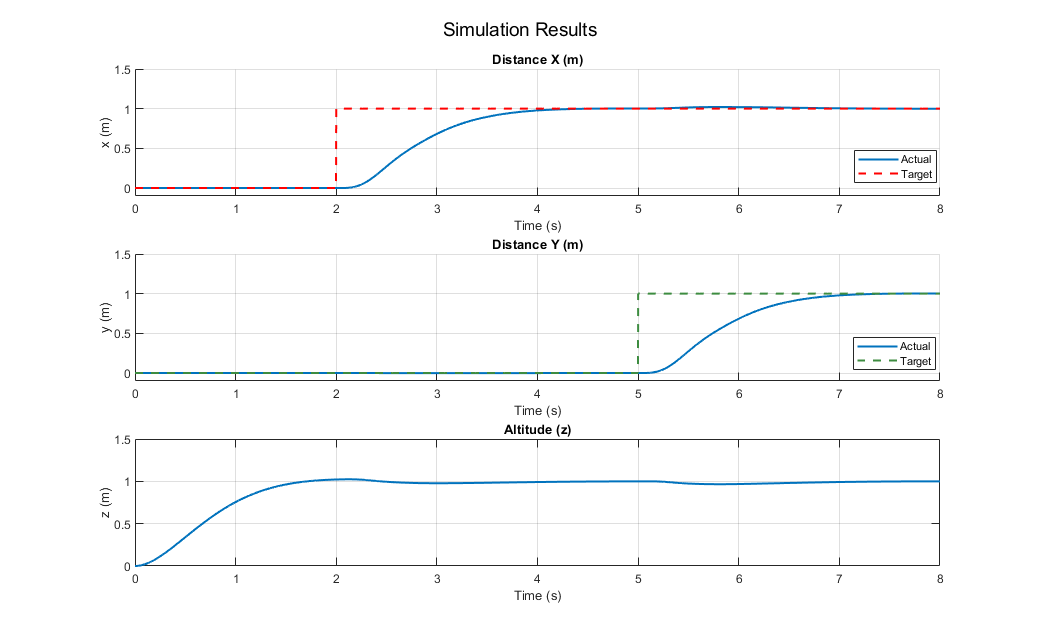
\includegraphics[width=1\textwidth]{LQR_Angles_Disp.png} % Specify image file and width
    \caption{LQR Controller cartesian coordinates} % Image caption
    \label{fig:LQR_Angles_Disp} % Label for referencing the image
\end{figure}
\begin{figure}[H] % 'h' places the image approximately where it appears in the code
    \centering
    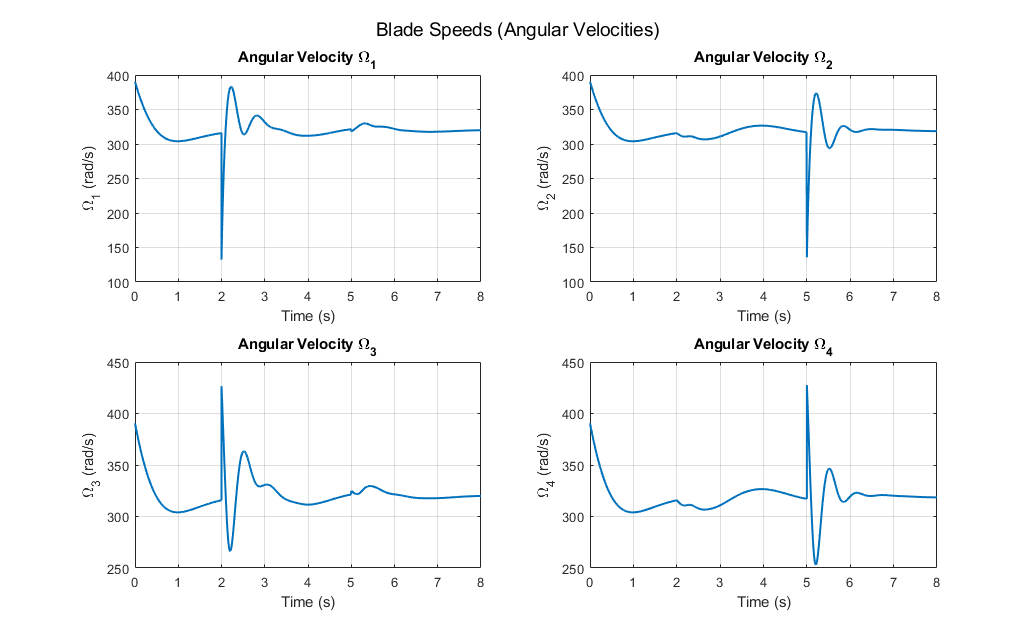
\includegraphics[width=1\textwidth]{LQR_Blade_Speeds.png} % Specify image file and width
    \caption{LQR Controller cartesian coordinates} % Image caption
    \label{fig:LQR_control_blade_speeds} % Label for referencing the image
\end{figure}
\noindent
It is evident that the controller we designed with the LQR performs better than the cascaded PID, both in how well it manages to follow the target, without overshoots, and in terms of actuator effort. We understand this from figure \ref{fig:LQR_control_blade_speeds}, since the changes in the speeds are much smoother, and we do not observe such large spikes in the speeds as those caused by the PID, which makes this control method, and specifically this controller, a preferable choice for controlling a physical drone. On a physical drone we would not be able to accelerate the rotors as easily, and in addition we would benefit from the lower energy consumption.
\\
\\
\noindent
Now we will design a specific trajectory and ask the drone's controller to move the system along this trajectory.
\begin{figure}[H] % 'h' places the image approximately where it appears in the code
    \centering
    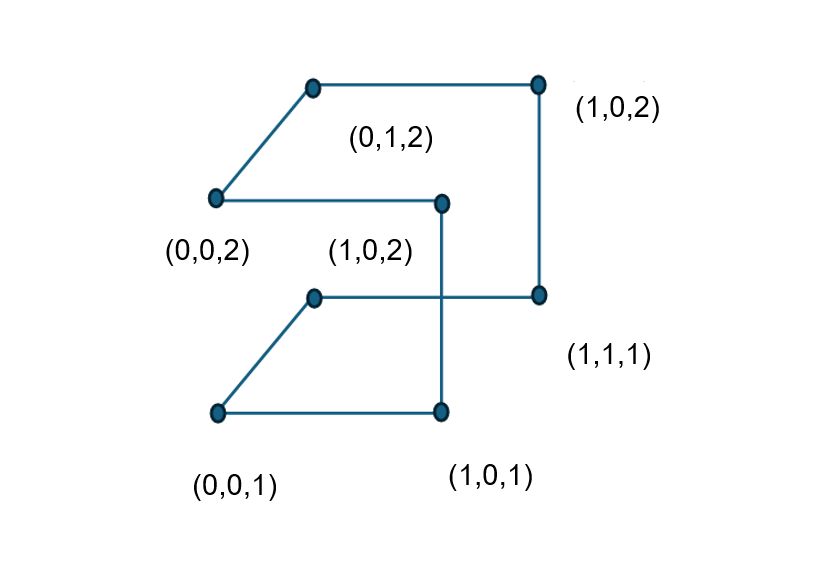
\includegraphics[width=0.5\textwidth]{Trajectory.png} % Specify image file and width
    \caption{Drone desired trajectory} % Image caption
    \label{fig:Trajectory} % Label for referencing the image
\end{figure}
The system response to the trajectory is shown below:
\begin{figure}[H] % 'h' places the image approximately where it appears in the code
    \centering
    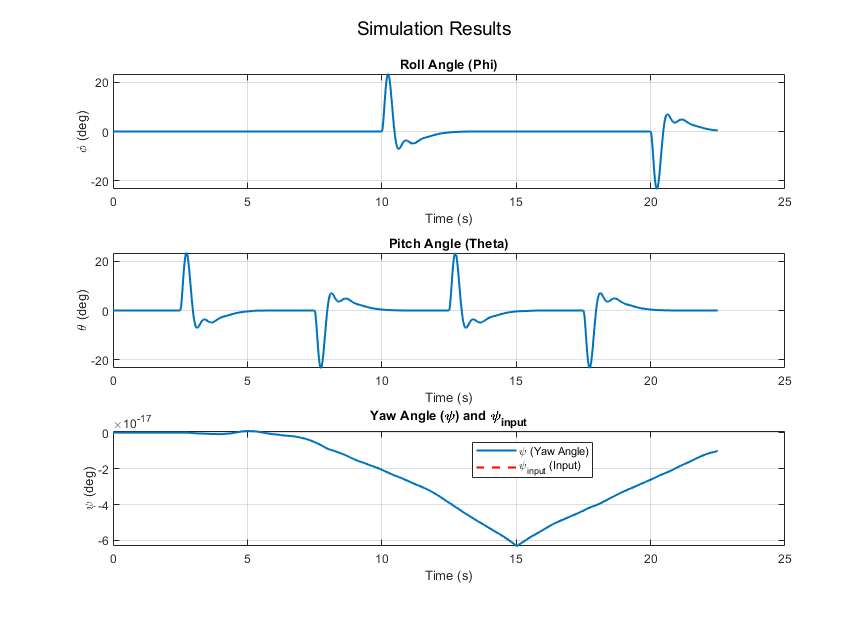
\includegraphics[width=0.95\textwidth]{LQR_Trajectory_Angles.png} % Specify image file and width
    \caption{Drone Euler angles following trajectory described in figure \ref{fig:Trajectory}} % Image caption
    \label{Trajectory_response_angles} % Label for referencing the image
\end{figure}
\begin{figure}[H] % 'h' places the image approximately where it appears in the code
    \centering
    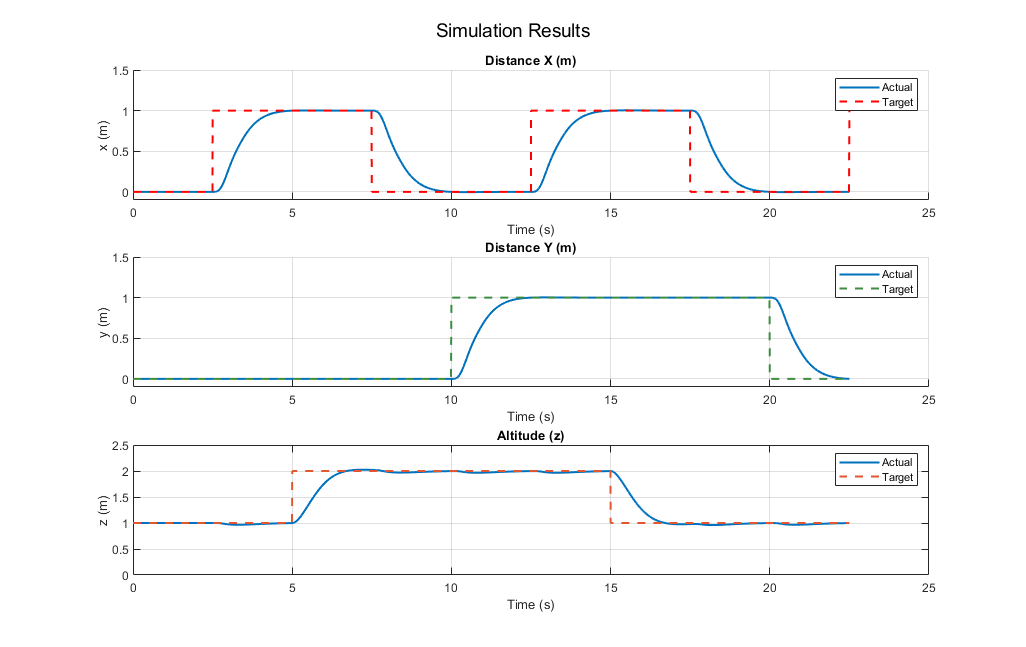
\includegraphics[width=0.99\textwidth]{LQR_T.png} % Specify image file and width
    \caption{Drone response cartesian coordinates \& coordinates of figure \ref{fig:Trajectory}} % Image caption
    \label{fig:Trajectory_response_disp} % Label for referencing the image
\end{figure}
\begin{figure}[H] % 'h' places the image approximately where it appears in the code
    \centering
    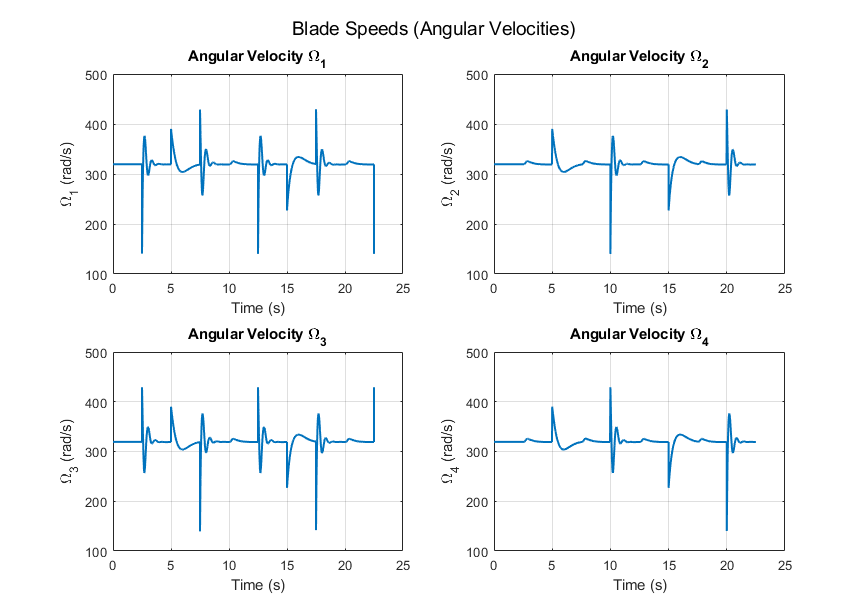
\includegraphics[width=1\textwidth]{LQR_Trajectory.png} % Specify image file and width
    \caption{Drone blade speeds following described in figure \ref{fig:Trajectory} } % Image caption
    \label{fig:LQR_Trajectory_full} % Label for referencing the image
\end{figure}
\noindent
We observe that the controller keeps the drone satisfactorily on the trajectory, without noticeable overshoots or undershoots, and without overworking the rotor motors. Figure \ref{fig:Trajectory_response_blade_speeds} shows exactly the trajectory that the drone ultimately follows, so that the controller's performance can be better appreciated.
\\
\\
\noindent
It becomes clear once again that the preferable method for designing controllers is through LQR and solving the corresponding Riccati equation, since both the tuning is easier and the final performance of the system is better. Especially for a system like this, where we have many state variables, when we designed the Cascaded PID controllers for the variables $x, y$ (thus 4 controllers), plus another 2 controllers for the variables $z, \psi$, we had to tune 18 parameters. With the LQR controller we had 16 parameters that required tuning, which, due to the assignment of weights to the state vector through the matrix Q, makes the tuning considerably easier than that of the PID.
\\
\\
\noindent
In any case, it is necessary to mention the significant advantage of the PID method, which is its particularly easy implementation and adaptation to the model. It requires no linearization or, more generally, any preprocessing of the system. It remains an easy and reliable way to quickly design functional controllers.

\begin{figure}[H] % 'h' places the image approximately where it appears in the code
    \centering
    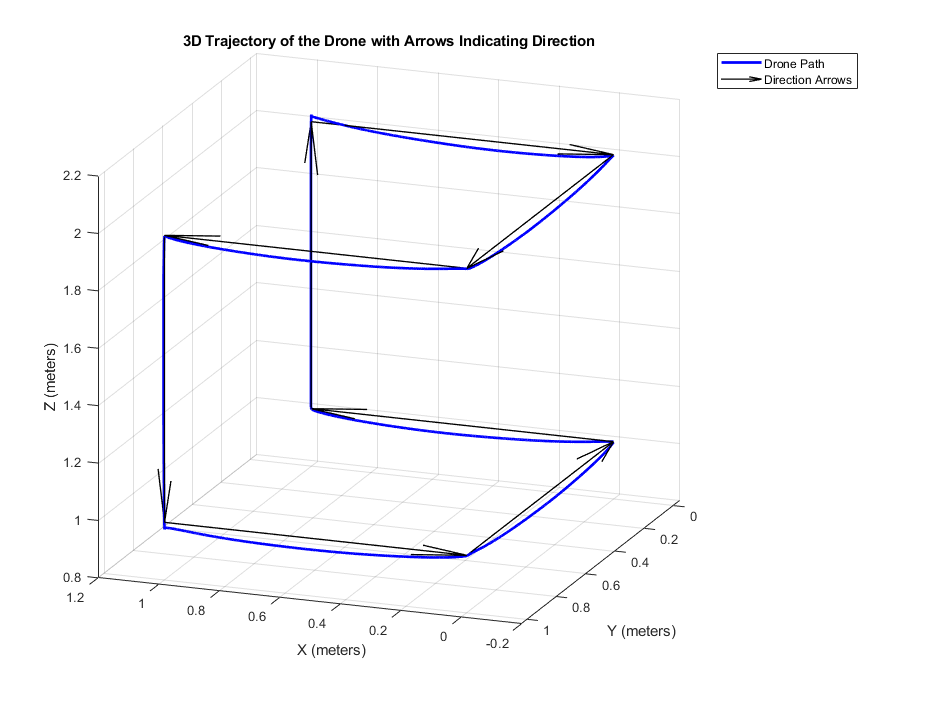
\includegraphics[width=1\textwidth]{Drone_Trajectory.png} % Specify image file and width
    \caption{Drone trajectory response for reference trajectory in figure \ref{fig:Trajectory} } % Image caption
    \label{fig:Trajectory_response_blade_speeds} % Label for referencing the image
\end{figure}
\end{document}
